% (c) Egor Osipov

\documentclass[a4paper,12pt]{article} % тип документа (report, book)
\usepackage[14pt]{extsizes}
\usepackage[left=2cm,right=2cm, top=2cm,bottom=2cm,bindingoffset=0cm]{geometry} % Настройки документа
\usepackage{pgfplots}
\usepackage{pgfplotstable}
\usepackage{tikz} 

%  Русский язык
\usepackage[T2A]{fontenc}			% кодировка
\usepackage[utf8]{inputenc}			% кодировка исходного текста
\usepackage[english,russian]{babel}	% локализация и переносы


% Математика
\usepackage{amsmath,amsfonts,amssymb,amsthm,mathtools} 

% Просто смайлики
\usepackage{wasysym}

%Вставка картинок
\usepackage{graphicx}
\graphicspath{./}
\DeclareGraphicsExtensions{.pdf,.png,.jpg}
\usepackage{float}

% Настройка абзацев
\usepackage{indentfirst}
%\setlength{\parindent}{5ex}
%\setlength{\parskip}{1em}

\begin{document} % начало документа

%Заговолок
\begin{titlepage}
\begin{center}
	\large{Московский физико-технический институт}\\
	\vspace{100px}
	\LARGE{Изучение лазерного гироскопа.}\\
	\vspace{30px}
	
\includegraphics[scale = 0.3]{fakt_logo.png}\\
\end{center}

\vfill
\begin{flushright}
	\text{Осипов Егор. Б03-005}\\
	\text{г. Долгопрудный}
\end{flushright}
\end{titlepage}

\newpage

\tableofcontents

\newpage

\section{Введение.}

В наше время наука об управлении движущимися объектами имеет особую
значимость. Важное место занимают автономные и полуавтономные (интегрированнные с GPS) инерциальные информационновычислительные системы,
использующие для определения углового пространственного положения лазерные гироскопы (ЛГ).

(ЛГ) обладают многими преимуществами перед традиционными механическими, среди которых необходимо назвать следующие:

1. ЛГ более устойчивы к климатическим и механическим воздействиям,
поскольку не имеют вращающейся массы.

2. ЛГ имеют малое время готовности.

3. Выходная информация об угле поворота в ЛГ выдается в цифровом
виде.

4. Количество включений и выключений ЛГ практически не ограничено.

В настоящее время ЛГ достигли точности лучше $0.001 ^\circ/\text{ч}$

В данной работе исследуются характеристики ЛГ нового поколения, в которых для вывода из зоны захвата вместо виброподвеса используется магнитооптическая (зеемановская) подставка, таким образом, ЛГ становится чисто оптическим прибором, не имеющим никаких движущихся механических частей, что обеспечивает ему дополнительные преимущества – более высокую устойчивость к жестким условиям эксплуатации и меньшие шумовые погрешности.

Итак, в данной работе мы изучим основные принципы работы и использования лазерного гироскопа, построенного на основе зеемановского кольцеового лазера.

\section{Теория лазерного гироскопа.}

\subsection{Лазерные гироскопы.}
 
\textbf{Лазерный гироскоп (ЛГ)} - оптический прибор для измерения угловой
скорости. Он обычно применяется в системах инерциальной навигации.

Первым оптическим гироскопом можно считать пассивный интерферометр
Саньяка. Трудность практического применения интерферометра Саньяка
обусловлена его малой чувствительностью, т.к. практически получаемая разность оптических путей значительно меньше длины волны.

Анализ принципа действия ЛГ лучше всего начать с описания вращающегося кольцевого интерферометра (см. рис.), свойства которого впервые были исследованы Саньяком.

% \begin{figure}
\begin{center}
    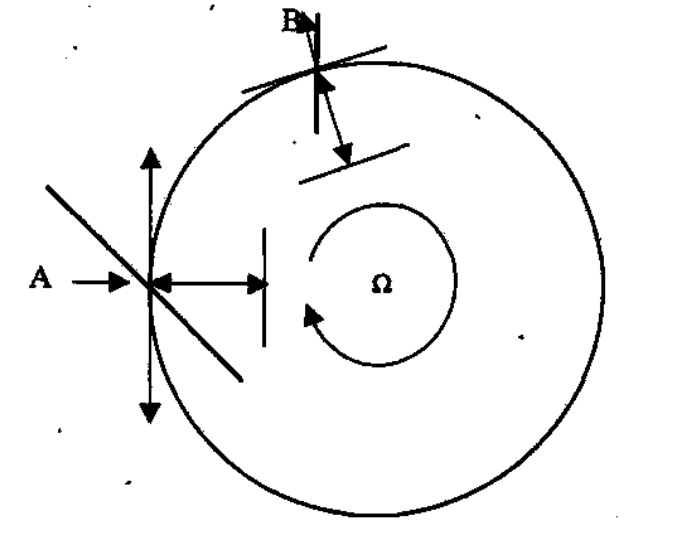
\includegraphics[scale=0.6]{pic1}\\
    \caption{Интерферометр Саньяка.}
    \label{pic1}
\end{center}
% \end{figure}

Если данный интерферометр вращается с угловой скоростью $\Omega$, то времена $t^+$ и $t^-$ прохода вдоль всего контура лучей, распространяющихся из точки А по и против часовой стрелки, будут разными:

\begin{equation}
    t^+ = (2\pi R ) / (c - R \Omega)
\end{equation}

\begin{equation}
    t^+ = (2\pi R ) / (c + R \Omega)
\end{equation}
где R -- радиус интерферометра, c -- скорость света в вакууме, $\Omega$ -- угловая скорость вращения интерферометра.

Разность данных времен составит:

\begin{equation}
    \vartriangle \!\! t = (t^+ - t^-) = 2 \pi R ((c + R \Omega - c + R \Omega)/
    (c^2 - R^2 \Omega^2)) =
    4 \pi \Omega R^2 / c^2 = 4 S \Omega / c^2
\end{equation}

Эта разность времен связана с разностью оптических
путей для распространения света в противоположных направлениях по замкнутому контуру, которая равна согласно выражению (3),

\begin{equation}
    \vartriangle \!\! L  = c \vartriangle \!\! t = 4 \pi \Omega R^2 / c
\end{equation}

Данное уравнение является основным при описании вращающегося интерферометра. Оно следует также из общей теории относительности, согласно
которой часы, движущиеся на вращающейся платформе, не синхронны по отношению к часам в инерциальном пространстве. Это различие обуславливает
разное время прохождения по замкнутому контуру для лучей, распространяющихся на вращающейся платформе в противоположных направлениях. Разность
времен определяется выражением:

\begin{equation}
    \vartriangle \!\! t = (2\Omega / C) \int \phi r^2 d\phi
\end{equation}
или
\begin{equation}
    \vartriangle \!\! t = 4A\Omega / c^2, \,\,\, \vartriangle \!\! L = 4A\Omega / c
\end{equation}
где А -- площадь, охватываемая оптическим контуром.

Данные выражения можно обобщить для произвольной конфигурации резонатора.

Существенного повышения чувствительности к угловым скоростям удается достичь путем применения активного интерферометра Саньяка – кольцевого
лазера (рисунок нижунок нижее).

Лазерный резонатор образуется тремя или четырьмя зеркалами, расположенными по углам полости в форме треугольника или квадрата. Два лазерных луча, генерируемые и усиливающиеся в полостях гироскопа, непрерывно циркулируют по резонатору в противоположных направлениях, условно обозначенных знаками + и -.

В кольцевом лазере с периметром L условие генерации можно записать в
виде:

\begin{equation}
    m \lambda_\pm = L_+ \text{ или } \nu_\pm = mc / L_+
\end{equation}
где m – число, характеризующее продольный тип колебаний ($m = 10^5...10^6$),
$\lambda_\pm$ и $\nu_\pm$ -- длины волн и частоты колебаний, соответствующие периметрам $L_\pm$ соответственно.

\begin{center}
    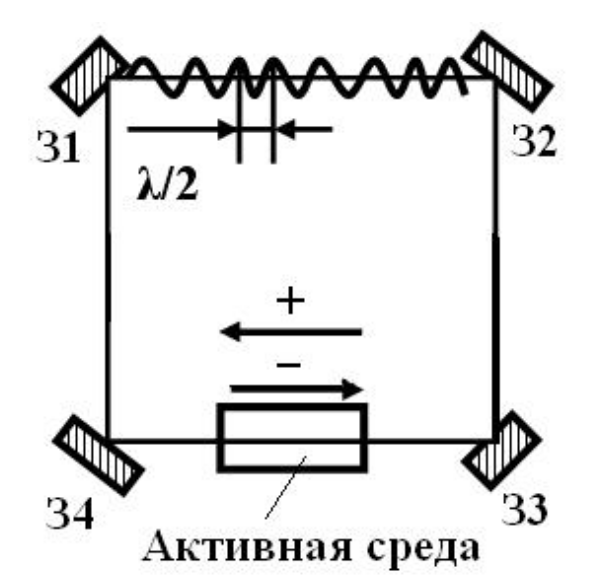
\includegraphics[scale=0.6]{pic2}\\
    \caption{Схема кольцевого лазера, образованного 4 зеркалами.}
\end{center}

Для автоматической настройки кольцевого лазера в резонанс в состав схем
его жизнеобеспечения входит схема регулировки периметра СРП.

В покоящемся лазере оптические пути $L_+$ и $L_-$ одинаковы и частоты
встречных лучей $\nu_+ = \nu_-$ . Ненулевая угловая скорость Ω вращения резонатора
приводит к неравенству оптических путей и соответственно к неравенству оптических частот, которые определяются в соответствии с отношением

\begin{equation}
    \vartriangle \!\! \nu / \nu = \vartriangle \!\! L / L
\end{equation}

В оптическом диапазоне частот малое изменение длины оптического пути приводит к значительному изменению частоты. В результате

\begin{equation}
    \vartriangle \!\! \nu = \frac {4S\Omega} {L \lambda} = k \Omega
\end{equation}
где S – площадь, охватываемая оптическим контуром, k – коэффициент пропор-
циональности.

В случае квадратного интерферометра со стороной квадрата $a$ формула (9)
примет вид:

\begin{equation*}
    \vartriangle \!\! \nu = \frac {a \Omega} {\lambda}
\end{equation*}

Измерения угловой скорости можно интерпретировать следующим образом. Стоячая волна, образующаяся в резонаторе суперпозицией встречных волн, сохраняет свое положение относительно инерциальной системы отсчета
независимо от углового перемещения резонатора. В таком случае при угловых
перемещениях гироскопа связанный с ним наблюдатель с помощью двух фотоприемников и счетчиков зафиксирует узлы или пучности стоячей волны электромагнитного поля, число которых в единицу времени даст разностную частоту $\vartriangle \! \! \nu$. При таком рассмотрении можно условно провести аналогию между лазерным и механическим гироскопом. В механическом гироскопе используется
инерция вращающейся массы, в лазерном гироскопе – инерция покоящейся
стоячей волны электромагнитного поля.

\subsection{Получение информации об угловой скорости вращения.}

Как уже отмечалось, информация о параметрах вращения получается измерением разности частот противоположно направленных волн, путем их гетеродинирования, которое заключается в пространственном совмещении волн и
выделении частоты биений.

Для реализации гетеродинного метода используется оптический смеситель, выполненный в виде призмы, в котором встречные волны создают
интерференционную картину. Интенсивности картины описываются следующим выражением

\begin{equation*}
    I = I_0 (1 + \cos(2 \pi \epsilon x / \lambda + \vartriangle \! \! \omega t +
    \phi)),
\end{equation*}
где $\vartriangle \! \! \omega = 2 \pi \! \! \vartriangle \! \! \nu$ -- угловая частота биения, $\epsilon = 2 n \theta$, n -- показатель преломления призмы, $\theta$ -- отклонение угла при вершине от $90^\circ$, $\phi$ -- постоянный сдвиг фаз.

Расстояние между полосами интерференционной картины равно $\lambda / \epsilon$. Для получения интерференционной картины с заданным расстоянием между полосами (1-3 мм) угол при вершине призмы должен отличаться от прямого на угол $\theta$, составляющий порядка 10-20".

Выходная информация считывается парой фотоприемников ФП1 и ФП2,
две фоточувствительные площадки которых выполнены в виде параллельных
полосок, помещенных в плоскость интерференционной картины и смещенных
относительно друг друга на четверть периода интерференционной картины.

В идеальном покоящемся ЛГ ($\Omega = 0$) частоты встречных волн равны ($\vartriangle \! \! \nu = 0$), и интерференционная картина неподвижна. При вращении лазера вокруг оси, перпендикулярной плоскости контура резонатора, называемой осью чувствительности, интерференционная картина перемещается со скоростью, пропорциональной $\vartriangle \! \! \nu$, в результате чего на выходах фотоприемников появляются
синусоидальные сигналы, сдвинутые по фазе на четверть периода. Эти сигналы
иногда называются сигналами SIN и COS. Направление вращения определяется направлением перемещения интерференционной картины.

Затем синусоидальные сигналы с помощью электронных схем преобразу-
ются в последовательность импульсов, число которых затем подсчитывается
реверсивным счетчиком Сч. На выходе счетчика образуется число N, которое
оказывается пропорциональным величине $\vartriangle \! \! \nu$ и, соответственно, угловой скорости $\Omega$. Знак числа N указывает направление вращения -- по часовой стрелке или против. ЛГ, таким образом, имеет цифровой выход.

ЛГ является интегрирующим устройством, измеряющим интегральный
угол поворота резонатора лазера в инерциальном пространстве за время съема
информации t:

\begin{equation}
    N = \int\limits_0^t \vartriangle \!\! \nu dt
\end{equation}

Обычно частота съема информации лежит в диапазоне 10-100Гц.

\begin{center}
    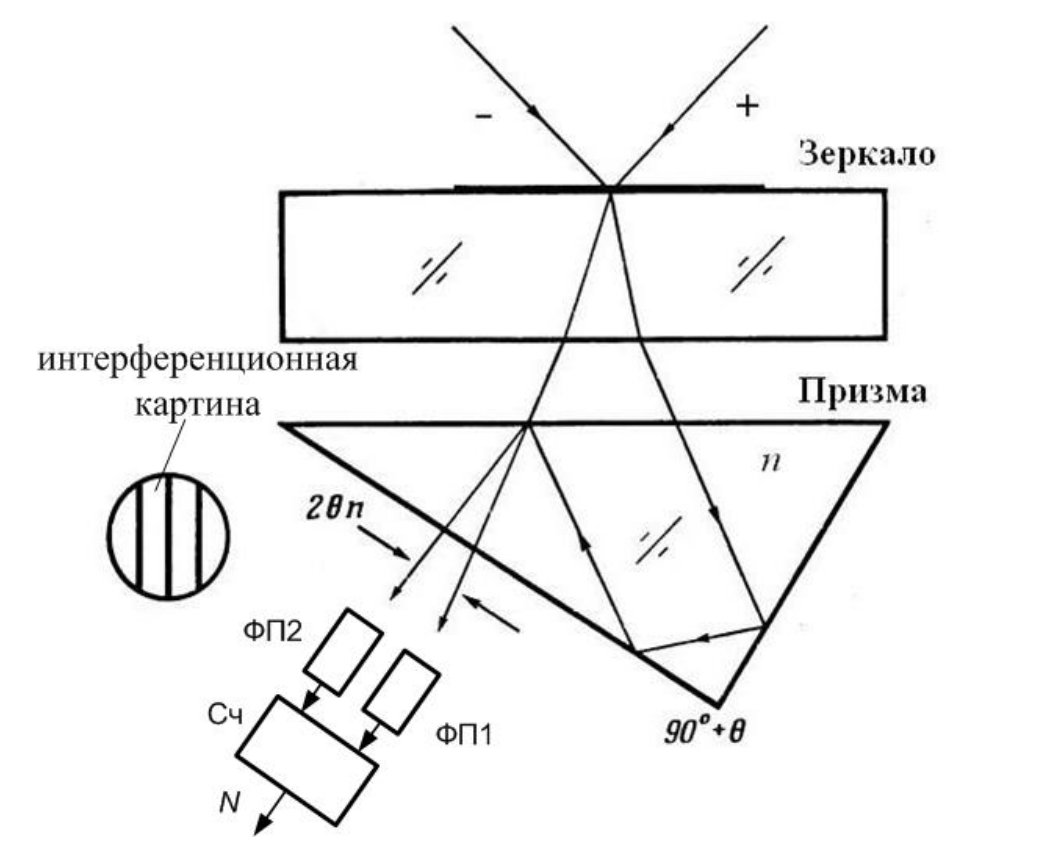
\includegraphics[scale=0.5]{pic3}\\
    \caption{Схема получения информации о параметрах вращения с лазерного гироскопа.}
\end{center}

\subsection{Погрешности цифрового гироскопа.}

Выходной, или частотной, характеристикой ЛГ является зависимость вида:

\begin{equation}
    \vartriangle \! \! \nu = f(\Omega),
\end{equation}
где $\vartriangle \! \! \nu$ -- измеренное значение разности частот встречных волн.

В идеальном случае это проходящая через ноль прямая. Однако в реальном
случае ЛГ присущи погрешности, которые изменяют вид выходной характеристики.

\begin{center}
    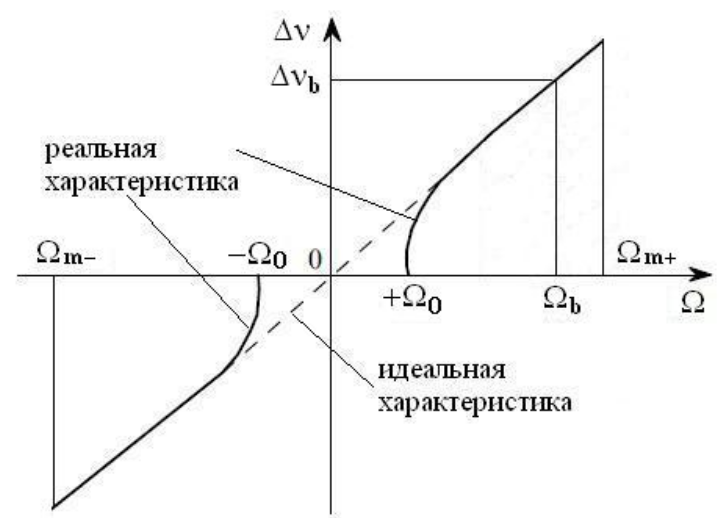
\includegraphics[scale=0.8]{pic4}\\
    \caption{Выходная характеристика лазерного гироскопа.}
\end{center}

Основными погрешностями ЛГ являются:

-- сдвиг и нестабильность нуля выходной характеристики;

-- нелинейность и нестабильность масштабного коэффициента;

-- синхронизация частот встречных волн в резонаторе.

Синхронизация встречных волн, или захват, является наиболее серьезным
недостатком ЛГ. Захват частот встречных волн проявляется в том, что при вращении ЛГ со скоростью, меньшей некоторого критического значения Ω 0 (порог
захвата), частоты противоположно направленных волн синхронизируются и частота биений на выходе фотоприемника становится равной нулю, то есть гироскоп перестает чувствовать вращение. На выходной характеристике образуется
зона нечувствительности к скорости вращения – «зона захвата» (рисунок выше).

Рассмотрим происходящие при захвате физические процессы более подробно. Наличие очень слабой шероховатости поверхности зеркал кольцевого
резонатора приводит к рассеянию части излучения (рисунок ниже). Как видно на рисунке, небольшая часть излучения $r_2E_2$ рассеивается в направлении распространения встречной волны $E_1$ . Следствием рассеяния является то, что в резонаторе появляется слабая связь между встречными волнами.

\begin{center}
    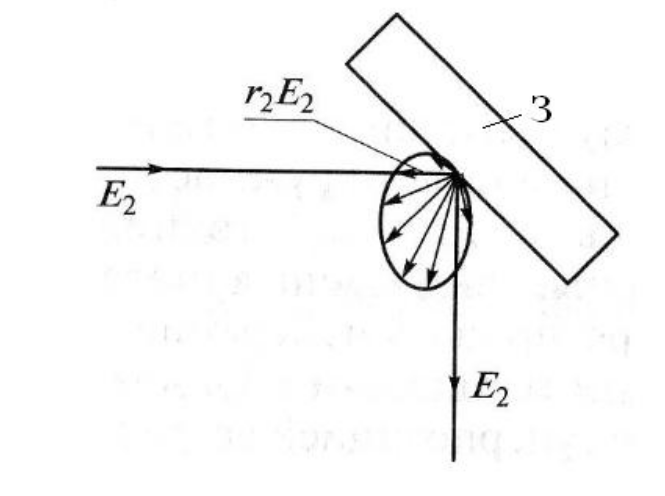
\includegraphics[scale=0.6]{pic5}\\
    \caption{Рассеяние световых волн.}
\end{center}

Представим встречные волны в виде фазовой диаграммы. Для этого электрические поля встречных волн записываются в виде

\begin{equation*}
    E(t) = E \cdot e^{i \phi(t)}
\end{equation*}

Средняя за период разность фаз полей встречных волн связана с разностью
их частот как

\begin{equation}
    \langle \phi_2(t) - \phi_1(t) \rangle_T = \Psi = \Omega \cdot t; \,\,\,
    \frac{d\Psi} {dt} = \Omega
\end{equation}

Представим векторы электрических полей встречных волн в системе координат, связанной с одним из векторов, например $E_1$. При таком представлении вектор $E_2$ вращается в выбранной системе координат со скоростью $d\Psi/dt$, а $\Psi$ является мгновенным значением угла между векторами $E_1$ и $E_2$. Рассеяние волны $E_2$ в волну $E_1$ с коэффициентом рассеяния $r_2$ и фазовым углом рассеяния $\epsilon_2$ приводит к тому, что вектор $E_1$ образуется сложением невозмущенного вектора $E_1^0$ и вектора $r_2E_2$, как это показано на рисунке ниже. За счет вращения вектора $E_2$ вектор $E_1$ оказывается промодулированным по фазе и по амплитуде на частоте $d\Psi/dt$. Поскольку в кольцевых лазерах фазовые изменения приводят к изменениям частоты в соответствии с соотношением $\frac{\alpha}{2\pi} = \frac{\delta \nu}{c/L}$, где $\alpha$ -- угол между направлениями векторов $E_1^0$ и $E_1$, то можно считать, что рассеяние волны $E_2$ ведет к изменению частоты волны $E_1$.

\begin{equation*}
    \delta \nu_1 = \frac {\alpha} {2\pi} \frac {c} {L}
\end{equation*}

\begin{center}
    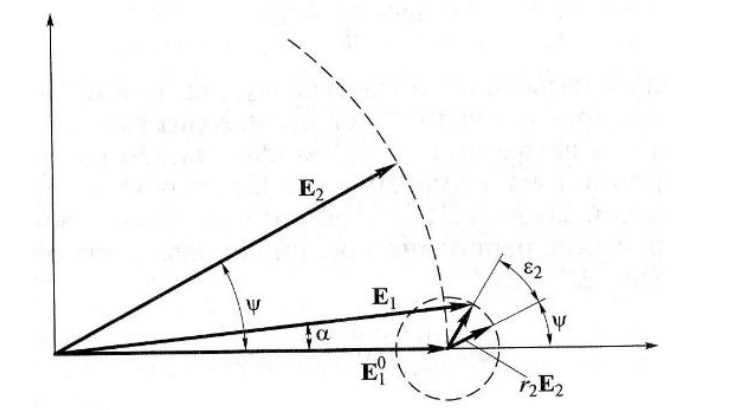
\includegraphics[scale=0.8]{pic6}\\
    \caption{Векторно-фазовая диаграмма затягивания частот при наличии обратного рассеяния.}
\end{center}

По диаграмме можно определить:

\begin{equation*}
    \sin(\alpha) = \frac{r_2 E_2} {E_1} \sin(\Psi + \epsilon_2)
\end{equation*}

Следовательно вместо уравнения (12) нужно записать:

\begin{equation}
    \frac {d\Psi} {dt} = \Omega - \Omega_0 \cdot \sin(\Psi + \epsilon_2),
\end{equation}
где $\Omega_0 = r_2 \frac{c}{L} \frac{E_2}{E_1}$ -- частота захвата.

В наиболее простом случае, когда $r_1 = r_2$, $\varepsilon_1 - \varepsilon_2 = \pi$, $E_1 = E_2$, получаем:

\begin{equation}
    \omega_0 = \frac {cr} {L}.
\end{equation}

Уравнение (13) имеет два решения. Одно решение справедливо при вы полнении неравенства $\Omega < \Omega_0$, что дает равенство разности встречных волн нулю:

\begin{equation*}
    \vartriangle \! \! \omega = \frac {d\Psi} {dt} = 0
\end{equation*}

Эта область называется областью захвата, или областью синхронизации
встречных волн. В ней происходит взаимная синхронизация частот встречных
волн, обусловленная рассеянием на элементах резонатора. Измерение угловых
перемещений, являющееся основной задачей ЛГ, в этой области невозможно.

Второе решение периодическое, оно справедливо при выполнении условия $\Omega > \Omega_0$:

\begin{equation}
    \vartriangle \! \! \omega = \frac {d\Psi} {dt} = \sqrt{\Omega^2 - \Omega_0^2}
\end{equation}

Выражение (15) отражает реальную характеристику ЛГ. В ней имеется зо на захвата, простирающаяся от $-\Omega_0$ до $+\Omega_0$ и имеющая ширину $2\Omega_0$.
Рядом с зоной захвата характеристика нелинейна и имеет гиперболический вид.

При интегральном рассеянии от всех четырех зеркал для лазера с периметром L = 16см получим $\vartriangle \! \! \nu_0 = (0,5 ... 1,7) \cdot 10^3 \text{Гц}$, что более чем на два порядка превышает расщепление частот встречных волн, вызванное вращением Земли (4,6 Гц). Отметим, что возможности уменьшения зоны захвата
чисто технологическими приемами в настоящее время практически исчерпаны, в связи с чем необходимо искать другие пути устранения ее влияния.

В настоящее время, чаще всего для уменьшения влияния связи встречных
волн на работу ЛГ, используется метод знакопеременного начального смещения, или так называемый метод частотной подставки. Идея метода состоит в
том, что при смешении рабочей точки выходной характеристики КЛ по периодическому закону лазер большую часть времени находится вне зоны захвата и
чувствует в это время входную скорость вращения (см. рис.). И лишь малую
часть периода изменения начального смешения КЛ находится в зоне захвата.
При этом очевидно, что чем больше амплитуда изменения смешения и чем
быстрее КЛ проходит через зону захвата, тем меньше влияние зоны захвата на
ЛГ. Оптимальной с этой точки зрения является прямоугольная форма закона
изменения начального смешения, так как в данном случае время нахождения в
зоне захвата равно нулю.

\begin{center}
    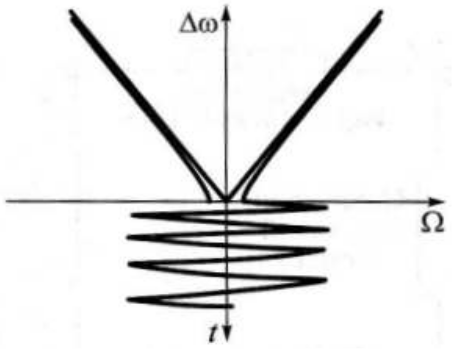
\includegraphics[scale=0.7]{pic7}\\
    \caption{Знакоопределенное смещение в лазерном гироскопе (частотная подставка)}
\end{center}

Знакопеременное начальное смешение реализуется обычно с помощью механических крутильных колебаний КЛ. В этом случае КЛ устанавливается на
специальную конструкцию, совершающую вынужденные колебания (с помощью электромагнита или пьезокерамических преобразователей) на собственной
резонансной частоте.

Метод частотной подставки в зеемановских кольцевых лазерах вследствие
их магнитной чувствительности реализуется путем создания переменного магнитного поля.

\subsection{Эффект Зеемана и знакоопределенная оптическая подставка.}

Для выведения рабочей точки ЛГ на линейный участок весьма
привлекательным является использование эффекта Зеемана. Такое использование оказывается возможным в кольцевых резонаторах с неплоским контуром и, как следствие этого, с круговыми поляризациями генерируемых волн.

Суть эффекта Зеемана состоит в том, что при наложении постоянного
продольного магнитного поля доплеровский контур усиления активной среды
расщепляется на два, симметрично сдвинутых относительно центра исходного
нерасщепленного контура.

\begin{center}
    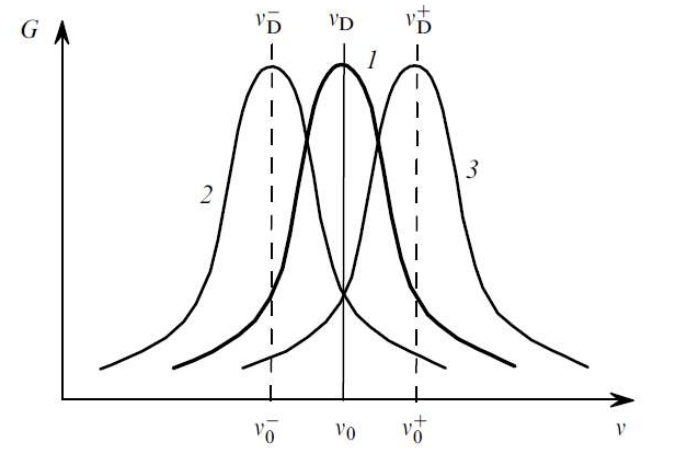
\includegraphics[scale=0.7]{pic8}\\
    \caption{Контур усиления активной газовой смеси в отсутствие магнитного
поля (1), низкочастотный (2) и высокочастотный (3) контуры, возникающие
при наложении продольного магнитного поля.}
\end{center}

Сдвиг определяется следующей формулой:

\begin{equation*}
    \vartriangle \! \! \nu^\pm_D = \pm \frac{g \beta H} {\hbar} << \vartriangle 
    \!\! \nu_D,
\end{equation*}
где g -- фактор расщепления; $\beta$ -- магнетон Бора; H -- напряженность магнитного поля, $\hbar$ -- постоянная Планка; $\vartriangle \! \! \nu_D$ -- ширина нерасщепленного контура. При этом более высокочастотный контур с центральной частотой $\vartriangle \! \! \nu^+_D = \nu_0 + g \beta H / \hbar$ усиливает волну только с правой круговой поляризацией, а более низкочастотный контур $\vartriangle \! \! \nu^-_D = \nu_0 - g \beta H / \hbar$ -- только с левой.

Если же смотреть вдоль волновых векторов волн, то усиливаться будет пара волн с одинаковой круговой поляризацией, например, только левой или правой, в зависимости от того, какая пара волн попала в исходный нерасщепленный контур усиления. Так, если в двухчастотном ЛГ на центр нерасщепленной
линии усиления была настроена частота резонаторных мод встречных волн с
правой круговой поляризацией, а вектор Н направлен вдоль канала контура по
часовой стрелке, то распространяющаяся по часовой стрелке волна «+» будет усиливаться контуром с частотой $\vartriangle \! \! \nu^+_D$, а волна «–», распространяющаяся против часовой стрелке, – с частотой $\vartriangle \! \! \nu^-_D$.

Если первоначальная настройка частоты резонаторных «+» и «–» мод на
максимум нерасщепленного контура усиления (при Н = 0) была произведена,
например, для пары встречных волн с правой круговой поляризацией, то при
наложении поля «+» мода сдвинется по направлению к центру высокочастотного контура ($\nu^+_D$), a «–» мода – к центру низкочастотного ($\nu^-_D$). Расщепление резонаторных мод определяется формулой

\begin{equation}
    \vartriangle \! \! \nu_b = 2 \delta \nu_D \frac{\vartriangle \!\! \nu_r}
    {\vartriangle \!\! \nu_D} \frac {G_0} {k} << \vartriangle \!\! \nu^\pm_D,
\end{equation}
где $\delta \nu_D = 2 \!\! \vartriangle \!\! \nu^\pm_D = 2g \beta H / hbar$ -- полное расщепление контуров усиления, $\vartriangle \!\! \nu_r$ -- ширина резонаторной моды, $G_0$ -- коэффициент усиления в максимуме контура усиления, $k$ – коэффициент потерь.

Таким образом, в покоящемся ЛГ вследствие наложения продольного магнитного поля возникнет разность частот генерации встречных волн, играющая
роль «частотной подставки», выводящей рабочую точку на линейный участок
частотной характеристики ЛГ.

Полагая $\vartriangle \!\! \nu_D = 1500 \text{МГц}$, $\vartriangle \!\! \nu_r = 1$МГц, $G_0 / k \approx 2G_0 / k \sim 2$, $H = 20$Э, получаем $\delta \nu_D \approx 72$МГц; $\vartriangle \!\! \nu_b = 192$кГц$ << \vartriangle \!\! \nu_D$. Поскольку, как указывалось ранее, полоса захвата $\vartriangle \!\! \nu_0 = (0,5...1,7) \cdot 10^3$Гц, то условие $\vartriangle \!\! \nu_0 >> \vartriangle \!\! \nu_b$ выполняется с большим запасом, что обеспечивает линейность участка частотной характеристики ЛГ вблизи новой рабочей точки $\vartriangle \!\! \nu_b$, которую можно теперь принять за нулевую точку отсчета.

На базе эффекта Зеемана была предложена знакопеременная магнитооптическая подставка, сводящаяся к знакопеременной периодической модуляции
параметров активной среды кольцевого лазера переменным магнитным полем.
Такая параметрическая модуляция, как нетрудно видеть из рисунка выше, приводит к
тому, что высокочастотный и низкочастотный контуры усиления периодически
меняются местами, вызывая тем самым периодическое изменение знака частотной подставки $\vartriangle \!\! \nu_b$. Частота модуляции $f_b$ обычно лежит в диапазоне 200-1000 Гц.

Надлежащей обработкой выходного сигнала, промодулированного частотой $f_b$, можно исключить (вычесть) его знакопеременную часть, оставив лишь
сигнал, обусловленный полезным невзаимным эффектом (т.е. вращением). Это
вычитание осуществляется за один период модуляции, то есть за время 15 мс, и
стабильность частоты подставки должна быть обеспечена именно за это время,
что технически относительно несложно, в то время как для ЛГ с постоянным
магнитным смещением такая стабильность должна быть обеспечена в течение
всего времени его работы.

В составе системы жизнеобеспечения ЛГ имеется блок частотной подставки (БЧП), который генерирует переменный ток с частотой $f_b$, пропускаемый через создающие магнитное поле катушки индуктивности, установленные
в лазерном резонаторе.

\section{Экспериментальное определение скорости вращения Земли, географической широты и азимута.}

ЛГ чувствителен к скорости вращения Земли. Если ЛГ установить на Северном полюсе и подсчитать за какое-либо время число импульсов, то оно будет пропорционально углу поворота нашей планеты, то есть определится временем измерения и полной скоростью вращения Земли, составляющей $\Omega_\text{З} = 15,04^\circ/\text{ч}$. Если тот же эксперимент повторить на экваторе, то число импульсов будет равно нулю, поскольку проекция скорости
вращения Земли на измерительную ось гироскопа будет равна нулю. Если же
измерительная ось ЛГ ориентирована горизонтально, то подсчитанное число
импульсов будет зависеть от ориентации прибора, то есть от угла между данным направлением и направлением на Север, называемого азимутом.

Эти факты обеспечивают возможность построения на базе ЛГ компаса –
лазерного гирокомпаса. С его помощью можно определять проекции скорости вращения Земли на оси системы координат, привязанной к корпусу прибора, географическую широту и азимут места установки.

Введем пять ориентаций измерительной оси ЛГ (рис. 1.9). При ориентации
1 измерительная ось направлена вверх, при ориентациях 2 – 5 – горизонтально.
Направление 2, азимут которого определяется в работе, и относительно его определяются положения 3 – 5.

\begin{center}
    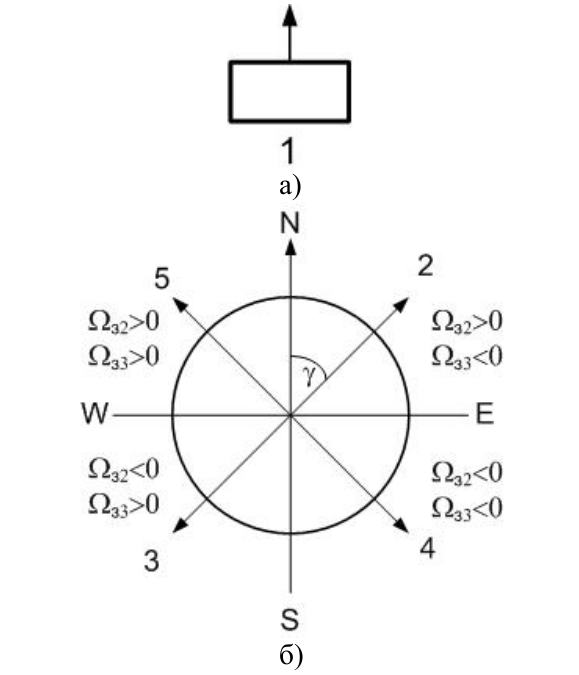
\includegraphics[scale=0.7]{pic9}\\
    \caption{Положения лазерного гироскопа при выполнении задания 3:
а) – вертикальное направление измерительной оси;
б) – горизонтальные направления измерительной оси}
\end{center}

Как видно из рисунка, направления 1,2,4 образуют систему координат,
привязанную к корпусу ЛГ. Направления 3 и 5 соответственно противоположны направлениям 2 и 4 и служат для внесения поправки, необходимость которой вызвана дрейфом нуля ЛГ при измерении скорости вращения Земли.

При проведении эксперимента ЛГ последовательно ставится в положения
1, 2, 3, 4, 5, и в каждом из положений в течение времени t подсчитываются им-
пульсы. В результате получаются числа $N_1$, $N_2$, $N_3$, $N_4$, $N_5$. Дрейф нуля рассчитывается после проведения эксперимента следующим образом

\begin{equation}
    \vartriangle \!\! \Omega = \frac {K(N_2 + N_3 + N_4 + N_5)} {4t},
\end{equation}
где K -- некоторый масштабный коэффициент.

Проекции скорости вращения Земли на оси системы координат гироскопа с
учетом поправки на дрейф находятся по формулам

\begin{equation}
    \Omega_\text{З1} = \frac {K \cdot N_1 - \vartriangle \!\! \Omega t}
    {t}
\end{equation}

\begin{equation}
    \Omega_\text{З2} = \frac {K \cdot N_2 - \vartriangle \!\! \Omega t}
    {t}
\end{equation}

\begin{equation}
    \Omega_\text{З3} = \frac {K \cdot N_3 - \vartriangle \!\! \Omega t}
    {t}
\end{equation}

Для расчета географической широты используется формула

\begin{equation}
    \varphi = \arcsin(\frac{\Omega_\text{З1}} {\Omega_\text{З}})
\end{equation}
где скорость вращения Земли известна.

Затем вычисляется синус и косинус угла азимута $\gamma$ по следующим формулам:

\begin{equation}
    \cos \gamma = \frac {\Omega_\text{З2}} {15,04 \cdot \cos \varphi}
\end{equation}

\begin{equation}
    \sin \gamma = \frac {\Omega_\text{З3}} {15,04 \cdot \cos \varphi}
\end{equation}

По знакам проекций скоростей вращения Земли можно в соответствии с рисунком (б) определить сектор, в которой находится азимут. Обратная тригонометрическая функция вычисляется по меньшему из значений, найденных по
формулам (22) и (23). В результате алгоритм окончательного определения азимута, измеряемого в радианах, выглядит следующим образом:

Если $\Omega_\text{З2} > 0$ и $\Omega_\text{З3} < 0$, то если $|\sin\gamma| < \cos\gamma$, то $\gamma = \arcsin(|\sin\gamma|)$, в противном случае $\gamma = \arccos(\cos \gamma)$.

Если $\Omega_\text{З2} < 0$ и $\Omega_\text{З3} < 0$, то если $|\sin\gamma| < |\cos\gamma|$, то $\gamma = \pi - \arcsin(|\sin\gamma|)$, в противном случае $\gamma = \pi - \arccos(|\cos\gamma|)$.

Если $\Omega_\text{З2} < 0$ и $\Omega_\text{З3} > 0$, то если $\sin\gamma < |\cos\gamma|$, то $\gamma = \pi + \arcsin(\sin\gamma)$, в противном случае $\gamma = \pi + \arccos(|\cos\gamma|)$.

Если $\Omega_\text{З2} > 0$ и $\Omega_\text{З2} > 0$, то если $\sin\gamma < \cos\gamma$, то $\gamma = 2\pi - \arcsin(\sin\gamma)$, в противном случае $\gamma = 2\pi - \arccos(\cos\gamma)$.

\end{document}
